The here-defined algorithm is based on classical graph algorithms. Its target is to find a suitable placement for distance restraints between two molecules $m_i$ and $m_j$ for a linked dual topology approach.

The following assumptions are made towards this process:
\begin{enumerate}
    \item $m_i$ and $m_j$ strongly overlap in the coordinate space; i.e., are aligned to each other
    \item optimal restraints placement for an MD simulation fulfills:
    \begin{enumerate}
        \item restrained atom pairs are maximally distributed over the two molecules
        \item restrained atoms have a minimal distance to each other ($d_{\text{res}} <= 1.0~\text{\AA}$)
        \item restraints are not hindering the molecule sampling
    \end{enumerate}
    \item given the number of required restraints $n_{\text{res}}$, it holds that $n_{\text{res}} << n_{\text{atoms}_{m_i}} \wedge~n_{res} << n_{\text{atoms}_{m_j}}$ 
\end{enumerate}
As a result of these assumptions, only relatively rigid areas of the molecules, such as ring-atoms, should be selected for the restraint search space. While restraining non ring atoms might be favorable for the distribution of the atoms over the molecules, it will be more likely to negatively affect the sampling behavior of the molecules.

\subsection{Assigning distance Restraints  to a pair of molecules}
\begin{figure}
    \centering
    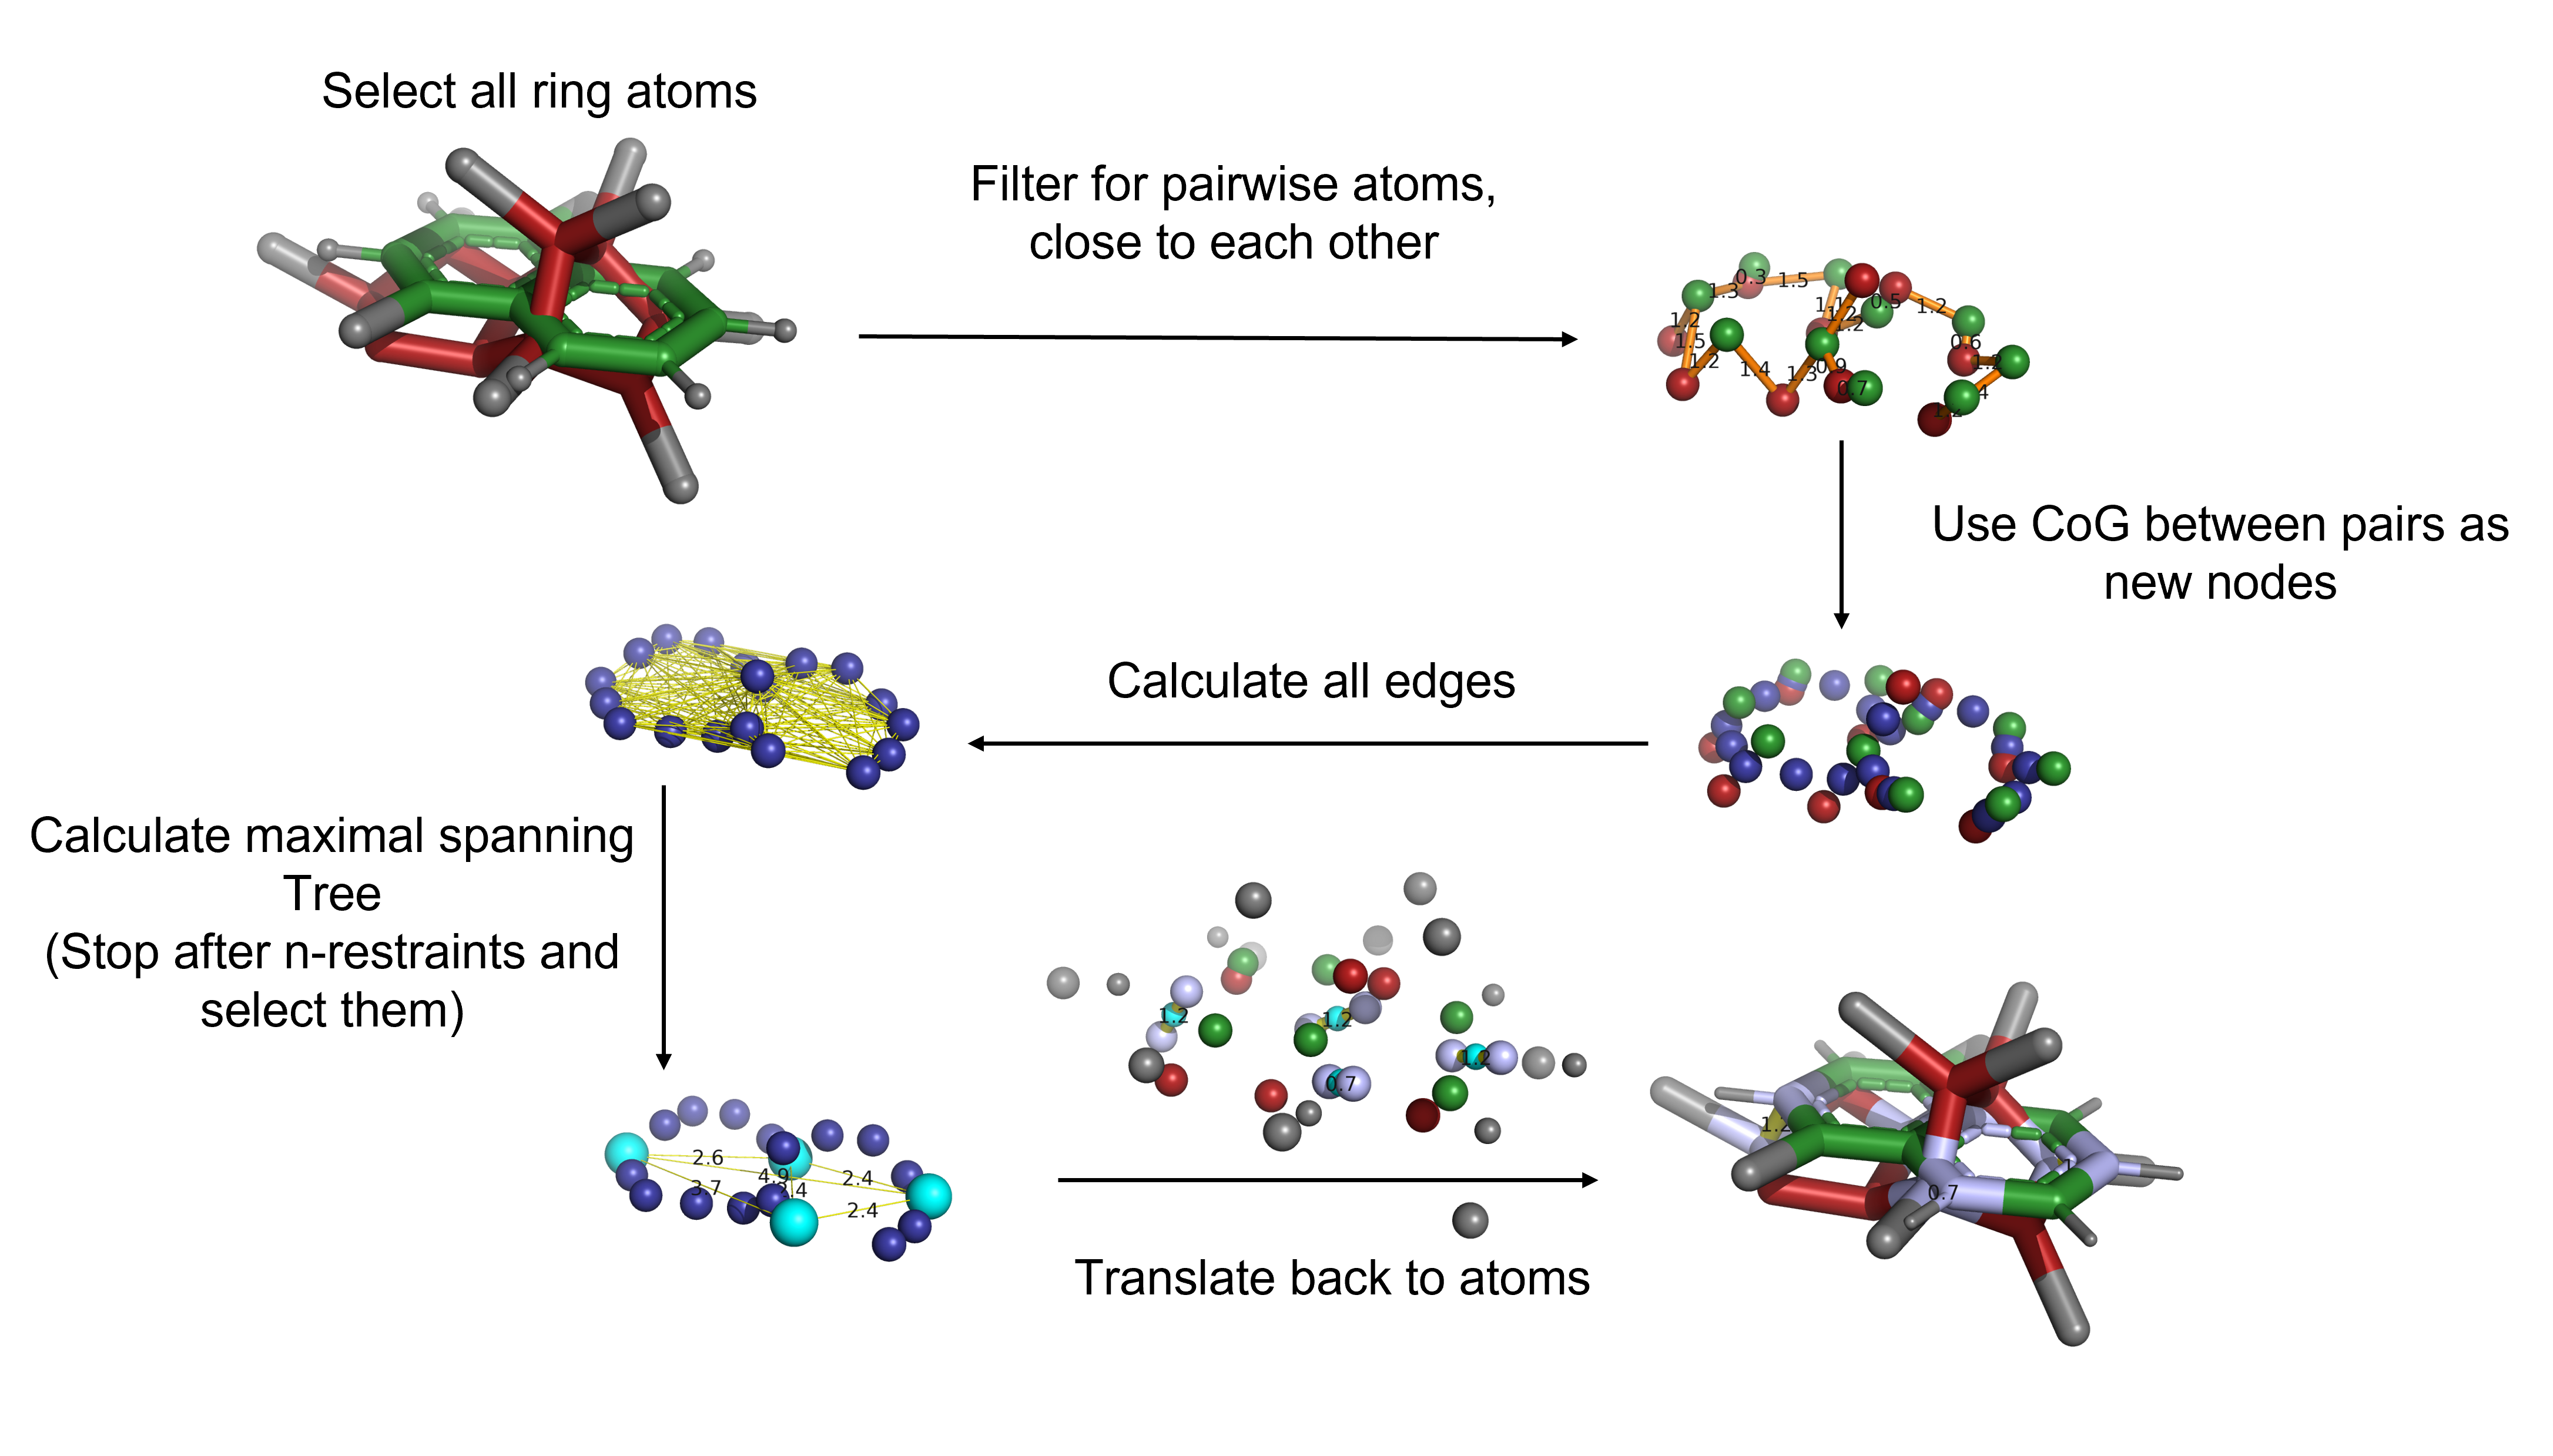
\includegraphics[width=\textwidth]{fig/theory/AlgorithmScheme.png}
    \caption{Algorithm scheme going stepwise through the algorithm}
    \label{fig:algorithmScheme}
\end{figure}

\subsubsection{Translation of the problem}
In order to be able to apply the algorithm to a pair of molecules, a set of pre-processing operations is required to translate the problem into a graph problem. 
The formulated approach is based on a graph representation of the restraint space. To be able to solve the graph problem of selecting a good set of atoms to form distance restrains, it needs to be translated into a graph fulfilling:
\begin{equation}
    G(N, E, \omega), E \subseteq \{\{x,y\}\mid x,y\in N\;{\textrm {and}}\;x\neq y\},
\end{equation}. \cite{}

with $N$ as a set of nodes, $E$ as a set of edges, and $\omega$ as a set of weights.

Here, we start with a molecule pair $mp$ consisting of a molecule $m_i$ and a molecule $m_j$ and their sets of atoms, $A_i$ and $A_j$, respectively, for which the relative free energy shall be determined. 

%%Alignment
In a first step, which will not be covered here in detail, the two molecules are aligned to each other, such that the overlap of the van der Waals surfaces of both molecules is maximal. This can be achieved using third-party tools such as the RDKit or PyMol. \cite{landrum2021, DeLano2020}

%%Filter
Next, the sets of possible atoms $A_i$ and $A_j$, that could be selected for the distance restraints are reduced to atoms  $A^{ring}_i$ and  $A^{ring}_j$, that are incorporated in molecule substructures forming a ring. 

%% Restraints with a Distance cutoff
$A^{ring}_i$ and  $A^{ring}_j$ are used to find potential restraints $R$,  with a user-defined cutoff distance $d_{a_i, a_j} \leq 1.0~\text{\AA}$ between the atoms. 
A potential restraint, therefore, is a pair of atoms $(a^{ring}_i, a^{ring}_j)$ that fulfills the distance criterion.

%% Building a Graph
All potential $R$ are used as nodes $N$ to construct a fully connected graph $G$. 
Each $r$ is represented by the center of geometry (COG) of the two involved atoms.
The undirected edges of the fully connected graph retrieve a weight as the euclidean distance $d_{\vec{r}_j,\vec{r}_i}=\omega_{ji}$ between two coordinates. 

\subsubsection{Solving the graph problem}
From the generated fully connected graph, only a selection of restraints is required to fulfill the assumptions. Many different algorithms could be applied to the graph in order to retain a set of restraints. Here, we decided to use a Min-Max decision scheme to build a spanning tree $R_{opt}$ within a greedy Prim-like approach.

%Algorithm Definition
%%bit more literature research
%initial move
The algorithm starts by picking the edge of $G$ with the largest $\omega_{ji}$/distance in the graph, i.e. the two restraints whose centers of geometry are the furthest away from each other. 

%iterate
%%update min
After this initial selection of two restraints for $R_{opt}$, the weights of $G$ are updated with the minimal distance of all $r$ in $R_{opt}$ to a respective node $n_i$. Subsequently, all edges and nodes are removed that contain atoms that are already selected in $R_{opt}$.

%% select max
After the edge update, the $e$ with maximal $\omega_{ji}$, and not connecting two nodes already in $R_{opt}$,  is added to  $R_{opt}$.

%%termination
This procedure is repeated till either all present nodes are connected or $|R_{opt}| = n_{res}$. 

\subsubsection{Mapping back}
The retrieved set of restraints $R_{opt}$ is translated back, such that the atoms forming the restraints can be selected and used to translate the distance restraints to a format usable for different MD packages like GROMOS or GROMACS. Additionally a JSON format is provided, allowing importing the results with any standardized JSON-Parser. \cite{Schmid2012, Abraham2015}


\subsubsection{Tie-Breaker}
Due to numerical accuracy and non-perfect alignment, small absolute differences in the priority calculation for the picking step were observed, leading to suboptimal results. These practical problems were solved by adding a tie-breaker that detects if multiple priorities in one iteration are within a range of $0.2$~\AA. 
Such a tie is broken by calculating the COG for all present restraints and using the distance to all current possible restraints as a secondary criterion. This distance should be maximal.


\subsection{Assigning distance Restraints to a multistate system}
In the case of multistate methods such as Replica Exchange Enveloping Distribution Sampling (RE-EDS) or $\lambda$-Dynamics, multiple molecules need to be restrained to each other. \cite{Sidler2016, knight2011} It was decided to form a ring of connecting restraints that links all molecules to two neighboring molecules in our approach.

The approach uses the described pairwise greedy approach to calculate all possible molecule pair restraints. The possible sets of restraints will be compared to each other by calculating the convex hull around the restraint coordinates. The convex hull volume (chv) is used to build up a fully connected graph connecting all molecules. The optimal connections are retrieved by applying a greedy algorithm, inspired by the Kruskal Algorithm, to the graph of ligand pairs (Figure \ref{fig: convexHull}). This algorithm picks the edges providing the largest chvs for chaining the pairs of restraints together. The following rules are applied during this: no node has larger connectivity than two, and no cycles in the generated graph are allowed. The cycle closure is achieved in the end by tying the loose chain ends together.

\begin{figure}[h]
    \centering
    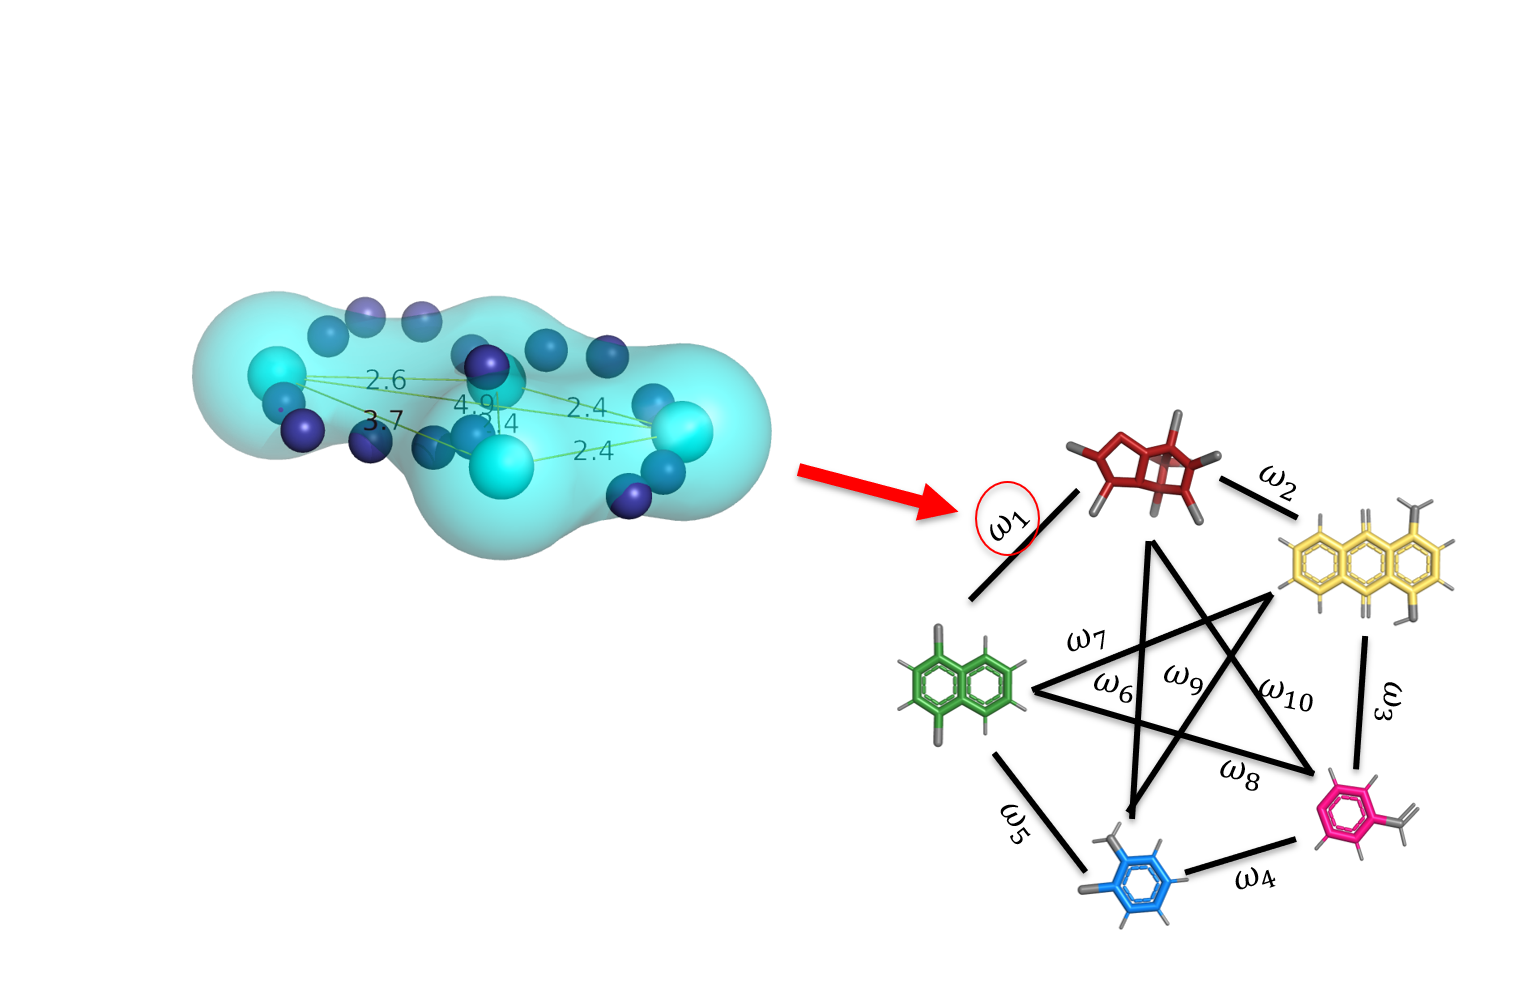
\includegraphics[width=\textwidth]{fig/theory/MultistateChainingScheme.png}
    \caption{Multistate Molecule chaining by maximizing the CHV}
    \label{fig: convexHull}
\end{figure}

\subsection{Free energy calculation methods}
In this work, two free energy calculation methods are applied with the linked dual topology approach.

\subsubsection{TI-Simulation}
Thermodynamic integration is a standard method for calculating free energies. It is used to sample a $\lambda$-dependent path between two end states A and B. The potential system energy is constructuted as follows:\cite{Kirkwood1935}
\begin{equation}
    V(\vec{r}; \lambda) = (1-\lambda) ~ V_A(\vec{r}) + \lambda ~ V_B(\vec{r})
    \label{eq: TI-Potential}
\end{equation}

In a simulation, state A is represented if $\lambda = 0$, and state B if $\lambda = 1$. Usually, the free energy is calculated as a path over multiple intermediate state simulations, in between the two extreme $\lambda$ values 0 and 1:
\begin{equation}
    \Delta F = \int^{1}_{0} \left< \frac{\delta V(\lambda)}{\delta \lambda} \right>_{\lambda} \,d\lambda
    \label{eq: TI-Integration}
\end{equation}

\subsubsection{RE-EDS}
%% Hamiltonian Construction
RE-EDS is a combination of Hamiltonian replica exchange (H-RE) and enveloping distribution sampling (EDS).\cite{Hansmann1997,Sugita2000, Christ2007, Sidler2016,Sidler2017,Ries2021} In EDS, a reference state Hamiltonian $V_R$ is sampled.\cite{Christ2007} $V_R$ combines $N$ end states as
\begin{align}
    V_R\left(\vec{r};s,\vec{E}^R\right) = -\frac{1}{\beta s}\ln\left[\sum\limits_{i=1}^N e^{-\beta s\left(V_i(\vec{r})-E_i^R\right)}\right]
\end{align}
with the smoothness parameter $s$ and a set of energy offsets $E_i^R$. 

The force on a particle $k$ can be calculated as \cite{Christ2008}

\begin{align}
    \vec{f}_k(t)=-\frac{\partial V_R(\vec{r}; s, \vec{E}^R)}{\partial \vec{r}_k} = \sum^N_{i=1}\frac{e^{-\beta s(V_i(\vec{r}) -E_i^R)}}{\sum^N_{j=1}{e^{-\beta s (V_j(\vec{r})-E_j^R)}}}  \left( -\frac{\partial V_i(\vec{r})}{\partial \vec{r}_k} \right) \,.
\end{align}

For high $s$ values, the sampling of the reference state is dominated by the state with the lowest $(V_i(\vec{r}) - E_i^R)$, whereas for low $s$ values, all states actively contribute to the system sampling resulting in the so called 'undersampling'. \cite{Riniker2011} 

EDS allows the calculation of the relative free energy difference of any end state pair in the system from a single simulation as

\begin{align}
    \Delta G_{BA} = -\frac{1}{\beta}\ln\frac{\langle e^{-\beta(V_B-V_R)}\rangle_R}{\langle e^{-\beta(V_A-V_R}\rangle_R} \, .
\end{align}

For EDS, an optimal choice of $s$ is essential to achieving good sampling of all end states in the system. RE-EDS reduces the difficulty of choosing an optimal $s$-value by simulating several replicas with different $s$-values and performing Hamiltonian replica exchanges.\cite{Sidler2016}
